\documentclass[tikz,border=6pt]{standalone}
% shared TikZ style for the diagrams (colours match the plots)
\usepackage[T1]{fontenc}
\usepackage{lmodern}
\usepackage{amsmath,amssymb}
\usepackage{tikz}
\usetikzlibrary{arrows.meta,positioning,fit,backgrounds,calc,shapes.misc,decorations.pathreplacing}
\definecolor{cBlue}{HTML}{2A78D6}
\definecolor{cOrange}{HTML}{EB6834}
\definecolor{cAqua}{HTML}{1BAF7A}
\definecolor{cViolet}{HTML}{6250D6}
\definecolor{cGreen}{HTML}{008300}
\definecolor{cGray}{HTML}{8F8D86}
\definecolor{cInk}{HTML}{0B0B0B}
\definecolor{cInk2}{HTML}{52514E}
\tikzset{
  box/.style={draw=#1!70!black, fill=#1!10, rounded corners=3pt, align=center, inner sep=4pt, font=\small, line width=0.6pt},
  box/.default=cGray,
  arr/.style={-{Stealth[length=2.4mm]}, line width=0.8pt, cInk2},
  lbl/.style={font=\scriptsize, text=cInk2, align=center},
}

\begin{document}
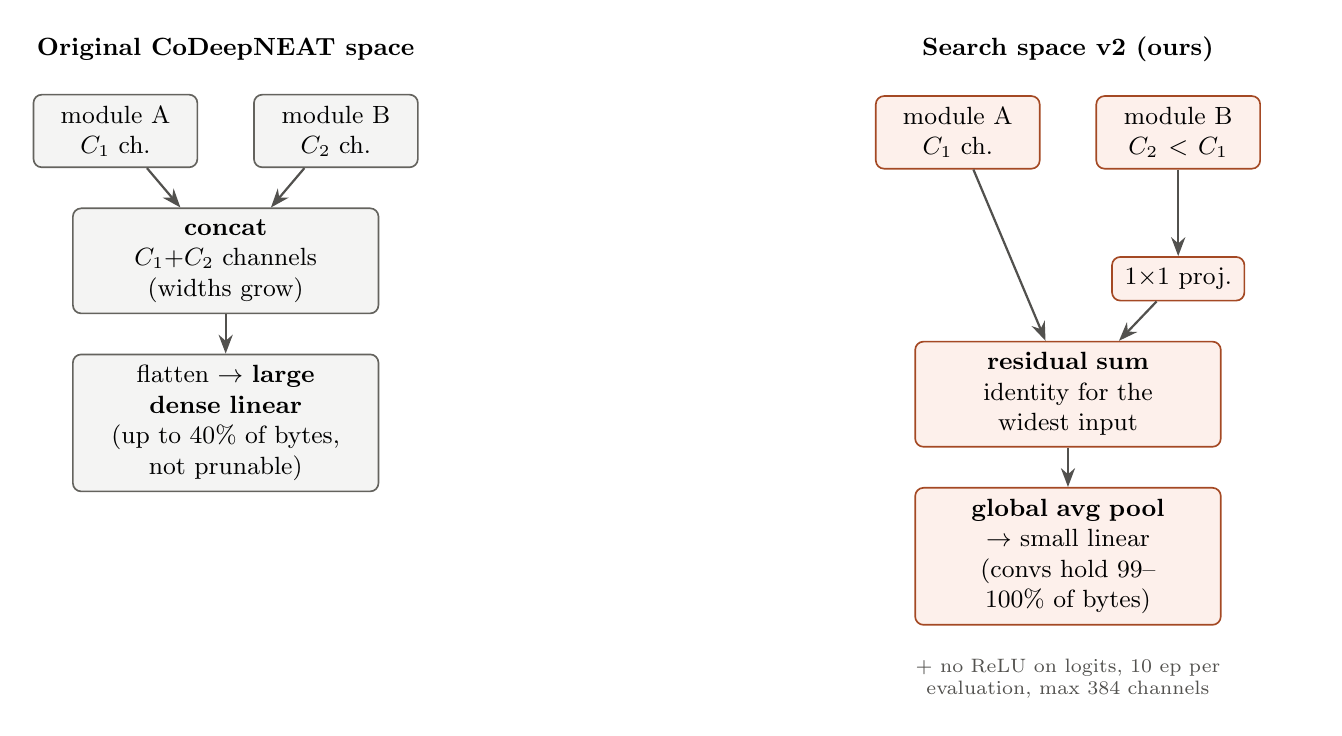
\begin{tikzpicture}[node distance=5mm and 6mm]
\node[font=\small\bfseries] (ta) {Original CoDeepNEAT space};
\node[box=cGray, below=3mm of ta, xshift=-14mm, text width=18mm] (a1) {module A\\$C_1$ ch.};
\node[box=cGray, below=3mm of ta, xshift=14mm, text width=18mm] (a2) {module B\\$C_2$ ch.};
\node[box=cGray, below=of a1, xshift=14mm, text width=36mm] (cat) {\textbf{concat}\\$C_1{+}C_2$ channels (widths grow)};
\node[box=cGray, below=of cat, text width=36mm] (fl) {flatten $\to$ \textbf{large dense linear}\\(up to 40\% of bytes, not prunable)};
\draw[arr] (a1)--(cat); \draw[arr] (a2)--(cat); \draw[arr] (cat)--(fl);
\node[font=\small\bfseries, right=62mm of ta] (tb) {Search space v2 (ours)};
\node[box=cOrange, below=3mm of tb, xshift=-14mm, text width=18mm] (b1) {module A\\$C_1$ ch.};
\node[box=cOrange, below=3mm of tb, xshift=14mm, text width=18mm] (b2) {module B\\$C_2<C_1$};
\node[box=cOrange, below=11mm of b2, text width=14mm] (pj) {$1{\times}1$ proj.};
\node[box=cOrange, below=of pj, xshift=-14mm, text width=36mm] (sum) {\textbf{residual sum}\\identity for the widest input};
\node[box=cOrange, below=of sum, text width=36mm] (gap) {\textbf{global avg pool} $\to$ small linear\\(convs hold 99--100\% of bytes)};
\draw[arr] (b2)--(pj); \draw[arr] (pj)--(sum); \draw[arr] (b1)--(sum); \draw[arr] (sum)--(gap);
\node[lbl, below=3mm of gap, text width=60mm] {+ no ReLU on logits, 10 ep per evaluation, max 384 channels};
\end{tikzpicture}
\end{document}
